\subsection{Source-Rule Development Test}

\label{app:docred_v2}

This version keeps the two prompts and four-action scheduler and adds
source rules for each document. A candidate marks a record as supported,
contradicted, or insufficient. The compiler checks an exact quote in
an original numbered sentence and saves character positions.
Augmentation sentences serve as generation hints. Insufficient evidence
or conflicting support and contradiction cause a skipped decision.
An allowed type rule leaves a source contradiction active.

Let $V(g;R)$ be the set of nonconflicting violations. Let $N$ be the
initial record count, using one for an empty input.
We use $G(g;R)=1-|V(g;R)|/N$ and coverage $C$ over initial records.
The graph-change term checks both graphs under updated rules:

\begin{align}
r_t={}&0.5\left[G(g_{t+1};R_{t+1})-G(g_t;R_{t+1})\right] \nonumber\\
&+0.5(C_{t+1}-C_t)-0.004a_t \nonumber\\
&-0.00002d_t-|V_{\mathrm{edit},t}|/N,
\end{align}

Here $a_t$ counts acquired responses and $d_t$ counts removed records.
$V_{\mathrm{edit},t}=V(g_{t+1};R_{t+1})\setminus V(g_t;R_{t+1})$ counts
edit-created violations. Acquisition can reveal an existing violation
with zero charge for creating it. A two-record synthetic test changes
discounted acquire--repair return from $-0.266519$ to $0.483481$
at discount $0.95$. This test checks reward accounting. The model judges
source support; the compiler checks the quote text.

Before calls, we fix the first ten development pairs, or 20 documents.
Each pair has one reference graph and one reference graph with added
endpoint or relation changes. The added count is $\lceil0.2|G^*|\rceil$.
References supply input construction and scoring. Prompts and policies
use public inputs. Each observation has 14 summaries and an action mask.
An episode allows four responses, two per strategy, and ten steps.
The removal guard blocks actions that would empty a nonempty graph.

\begin{table}[t]
\centering
\caption{Source-rule test on ten fixed document pairs. F1 and facts kept are episode means. Lost counts removed reference facts. Schedules are fixed.}
\label{tab:docred_source_pilot}
\small
\begin{tabular}{lrrr}
\hline
Schedule & F1 (\%) & Facts kept (\%) & Lost \\
\hline
Stop & 94.42 & 100.00 & 0 \\
Acquire then repair & 94.59 & 98.34 & 4 \\
Repair when feasible & 91.63 & 93.51 & 18 \\
Uniform feasible & 94.42 & 100.00 & 0 \\
\hline
\end{tabular}
\end{table}

The 40 outputs use 40 Gemma requests. They compile to 357 type rules,
61 source-support rules, and 6 source-contradiction rules.
Source rules trigger removal in 4 of ten episodes. The fixed expansion
check requires at least two such episodes, higher mean reference F1,
and at least 99\% reference facts kept. This version ends at that check.
Scores measure reference recovery and injected-item removal.
Saved-output replay uses zero API calls.

\begin{figure*}[t]
\centering
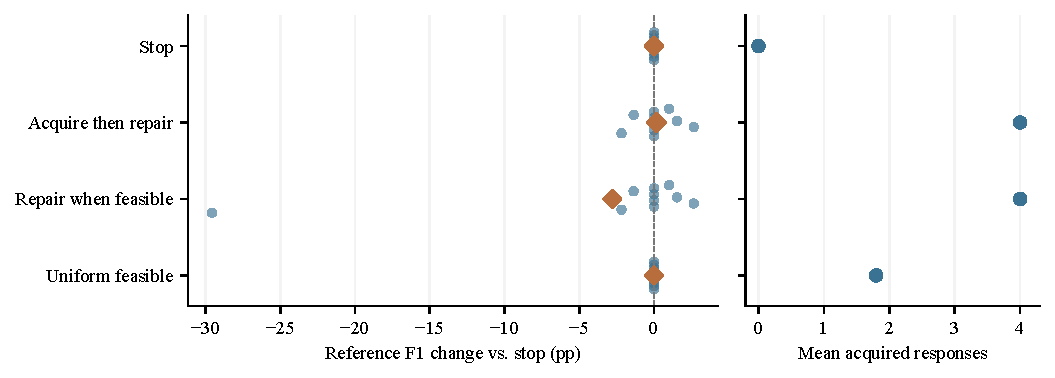
\includegraphics[width=0.94\textwidth]{figure/experiments/docred_source_pilot.pdf}
\caption{Source-rule replay. Dots show ten episode F1 changes from stop; diamonds show their mean. The right panel counts acquired saved responses.}
\label{fig:docred_source_pilot}
\end{figure*}
